\documentclass[11pt]{article}

\usepackage[utf8]{inputenc}
\usepackage{tabularx}
\usepackage{hyperref}
\usepackage{array}  
\usepackage{graphicx}
\usepackage{geometry} 
\usepackage{fancyhdr} 
\usepackage{tikz}
\usepackage{ragged2e}
\usepackage{anyfontsize}
\usepackage[table,xcdraw]{xcolor}
\usepackage{tabularx, etoolbox} 
\usepackage{eso-pic}
\usepackage{float}

\graphicspath{{images}}
%\graphicspath{{../images/}}

\setcounter{secnumdepth}{4}


%cambio misure della pagina
\geometry{a4paper,left=25mm,right=25mm,top=25mm,bottom=25mm}
%ebdfc7
\definecolor{colorePie}{HTML}{ebdfc7}
\pagestyle{fancy}
\fancyhf{}
\renewcommand{\headrulewidth}{0.4pt}
\lhead{
    \parbox[c]{1cm}{\includegraphics[width=1.1cm]{Sevenbitslogo.png}}
}
\rhead{\textcolor[HTML]{9e978a}{ ANALISI DEI REQUISITI v0.2.7}
}
\setlength{\headheight}{25pt}
\cfoot{\thepage}


\renewcommand*\contentsname{Indice}
\renewcommand{\listfigurename}{Elenco delle figure}
\renewcommand{\listtablename}{Elenco delle tabelle}

\begin{document}

% Pagina del titolo
\begin{titlepage}
    \setcounter{page}{0}
    \centering
    % Inserisci il logo del gruppo (modifica il percorso dell'immagine)
    \includegraphics[width=7.2cm]{Sevenbitslogo.png} \\[2cm] 
    
    % Titolo
     {\fontsize{40}{40}\bfseries Analisi dei Requisiti}\selectfont \\[3.9em]
    
    % Sottotitolo
    {\huge NearYou\\ \vspace{3mm }Smart custom advertising platform} \\[2.7em]
    
    % Email del gruppo
    {\large sevenbits.swe.unipd@gmail.com} \\[3em]
    
    % Spazio per il logo dell'università
    \hfill
      
    \AddToShipoutPictureBG{ % Imposta il triangolo con logo
        \ifnum\value{page}=0
        \begin{tikzpicture}[overlay]
        
            % Definisce un triangolo blu in basso a destra
            \fill[colorePie] 
                (current page.south east) -- ++(-9cm,0) -- ++(9cm,9cm);
            
            % Inserisce il logo all'interno del triangolo
            \node[anchor=south east, xshift=-0.3cm, yshift=0.3cm] at (current page.south east) {
                \includegraphics[width=4.5cm]{LogoUnipd.png}
            };
        \end{tikzpicture}
        \fi
    }
        
\vfill % Aggiunge spazio verticale per centrare il contenuto
\end{titlepage}
\newpage
\clearpage
\setcounter{page}{1}

\centering\textbf{Registro modifiche}\\
\vspace{2mm}
\begin{tabularx}{\textwidth}{|l|l|l|l|X|}
\hline
\textbf{Versione} & \textbf{Data} & \textbf{Autore} & \textbf{Verificatore} & \textbf{Descrizione} \\
\hline
0.2.7 & 2024-12-02 & Manuel Gusella & Giovanni Cristellon & Aggiunta di UC1.3.2 e RF10 \\
\hline
0.2.6 & 2024-11-30 & Federico Pivetta & Giovanni Cristellon & Aggiunta di RQ05, RQ06, RV05, RP02, indice tabelle e nuovo stile tabelle \\
\hline
0.2.5 & 2024-11-29 & Uncas Peruzzi & Leonardo Trolese & Aggiunta di UC5, aggiornati requisiti di qualità, vincolo e tabella \\
\hline
0.2.4 & 2024-11-28 & Federico Pivetta & Leonardo Trolese & Aggiunta di UC1.3, UC1.3.1, RF02, RF04 e RF05, correzione tabella requisiti funzionali \\
\hline
0.2.3 & 2024-11-26 & Leonardo Trolese  & Federico Pivetta & Correzioni minori grammaticali e di contenuto \\
\hline
0.2.2 & 2024-11-25 & Leonardo Trolese  & Federico Pivetta & Aggiunta di UC3, UC3.1, UC3.2, UC4, RF01 e RF08 \\
\hline
0.2.1 & 2024-11-23 & Manuel Gusella  & Federico Pivetta & Aggiunta di UC1.2, UC2, RF03 e RF06\\
\hline
0.2.0 & 2024-11-21 & Uncas Peruzzi  & Federico Pivetta & Migliorie varie e inizio redazione sez.\ref{sec:casi-uso} \\
\hline
0.1.1 & 2024-11-15 & Uncas Peruzzi  & Riccardo Piva & Redazione sez.\ref{sec:intro} e sez.\ref{sec:descrizione} \\
\hline
0.1.0 & 2024-11-14 & Uncas Peruzzi  & Riccardo Piva & Inizio redazione del documento\\
\hline
\end{tabularx}

\newpage
\tableofcontents
\newpage
\listoffigures
\newpage
\listoftables

\newpage
\begin{justify}

\section{Introduzione}
\label{sec:intro}

\subsection{Scopo del documento}

Il seguente documento ha l'obiettivo di fornire una descrizione accurata dei casi d'uso e dei requisiti riguardanti il progetto \textit{"NearYou - 
Smart custom advertising platform"} concernenti il Capitolato C4 proposto dall'azienda SyncLab e aggiudicato al gruppo dal committente.


\subsection{Glossario}
Con l'intendo di evitare ambiguità interpretative del linguaggio utilizzato, viene fornito un Glossario che si occupa di esplicitare il significato dei termini che riguardano il contesto del progetto. I termini presenti nel glossario sono contrasegnati con una \textit{G} a pedice : Termine$_G$.\\
Le definizioni sono presenti nell'apposito documento \textit{Glossario.pdf}


\subsection{Riferimenti}

\subsubsection{Riferimenti normativi}
\begin{itemize}
    \item[-] ISO/IEC/IEEE 29148:2018(E) \\
    \textcolor{blue}{\texttt{\url{https://ieeexplore.ieee.org/stamp/stamp.jsp?tp=&arnumber=8559686}}}
    
    \item[-] Regolamento del progetto didattico  \\
    \textcolor{blue}{\texttt{\url{https://www.math.unipd.it/~tullio/IS-1/2024/Dispense/PD1.pdf}}}
    
\end{itemize}
\subsubsection{Riferimenti informativi}
\begin{itemize}
    \item[-] Capitolato C4 - NearYou - Smart custom advertising platform\\
    \textcolor{blue}{\texttt{\url{https://www.math.unipd.it/~tullio/IS-1/2024/Progetto/C4p.pdf}}}
    \item[-] Analisi dei Requisiti - SWE 2024-25\\
    \textcolor{blue}{\texttt{\url{https://www.math.unipd.it/~tullio/IS-1/2024/Dispense/T05.pdf}}}
    \item[-] Analisi e descrizione delle funzionalità: Use Case e relativi diagammi - SWE 2024-25\\    
    \textcolor{blue}{\texttt{\url{https://www.math.unipd.it/~rcardin/swea/2022/Diagrammi\%20Use\%20Case.pdf}}}
    \item[-] Verbali Interni
    \item[-] Verbali Esterni
    
\end{itemize}

\newpage
\section{Descrizione del prodotto}
\label{sec:descrizione}
\subsection{Obiettivi del prodotto}
Il prodotto software da sviluppare, ha il principale obiettivo di generare annunci personalizzati per l'utente, sulla base della sua profilazione e posizione in tempo reale sulla mappa, tramite l'utilizzo degli LLM, nel momento in cui si trovi su un veicolo (dotato di display). Il risultato desiderato, prevede di proporre agli utenti esclusivamente annunci finalizzati a catturare il loro interesse, con il fine di massimizzare il tasso di engagement.

\subsection{Ambito del prodotto}
Il campo di applicazione del prodotto software \textit{NearYou - 
Smart custom advertising platform}, è focalizzato su una serie di clienti che offrono un servizio di renting di mezzi di trasporto, dotati di display, nei quali durante l'itinerario di viaggio vengano presentate pubblicità mirate in base a diversi fattori:
\begin{itemize}
    \item [-] sensori di posizione (GPS);
    \item [-] informazioni date dagli utenti in fase di iscrizione;
    \item [-] informazioni di stato fisico dell’utente.
\end{itemize}

\subsection{Panoramica del prodotto}
\subsubsection{Prospettiva generale del prodotto} 
In questa sezione vengono elencate tutte le interfacce di sistema che possono interagire con il prodotto \textit{Near You}.

\paragraph{Interfacce utente}\mbox{}\\
\textit{Near You} è un prodotto che genera messaggi pubblicitari personalizzati per l'utente. Questi messaggi sono pensati per essere visualizzati mediante un'interfaccia utilizzabile su display touchscreen, con la quale l'utente può interagire visivamente e fisicamente; tuttavia con la proponente è stato stabilito che tale interfaccia utente 
è un requisito opzionale poichè può essere facilmente ottenuta a partire dalla dashboard dell'utente privilegiato mediante un semplice filtro.\\
In ogni caso, nell'ambiente di sviluppo del prodotto, il display è emulato tramite una web-app che presenta una mappa interattiva sulla quale vengono visualizzate pubblicità associate ai punti di interesse. Per l'utente 
privilegiato, che offre il servizio di renting, è invece presente, come accenato prima, una dashboard nella quale è possibile visualizzare la mappa, con tutte le posizioni live dei mezzi e i vari punti di interesse, 
generati dal software sottostante.

\paragraph{Interfacce hardware}\mbox{}\\
Il prodotto sviluppato sfrutta i dati monitorati e acquisiti da sensori, nel contesto di sviluppo saranno dati generati attraverso simulazioni reali. Il display touchscreen, corrisponderà a una web-app accessibile da un web browser.\\
Come risultato di quanto detto lo sviluppo del progetto non avviene con elementi hardware fisici.

\subsubsection{Funzionalità del prodotto}
Il prodotto software dovrà garantire le seguenti caratteristiche:
\begin{itemize}
    \item [-] generazione e salvataggio di dati personali relativi a utenti fittizi, su cui dimostrare il funzionamento del software.
    \item [-] simulazione dati provenienti dai sensori GPS, nel caso del percorso effettuato dall'utente, deve corrispondere a coordinate di itinerari che esistono realmente.
    \item [-] separazione del flusso di dati generato dai simulatori, tramite l'utilizzo di un broker opportuno, facilitando di fatto la gestione delle informazioni tra i diversi componenti del sistema.
    \item [-] individuazione dei punti di interesse specifici, sfruttando LLM, che prende in input i dati di profilazione e posizione simulati.
    \item [-] serializzazione dei dati precedentemente menzionati, in un database adatto alla tipizzazione degli input e performante in tale contesto.
    \item [-] acquisizione e elaborazione dei dati dei sensori per mezzo di uno strumento adatto allo stream processing, per fornirli in pasto al framework di generative AI.
    \item [-] fornire un'interfaccia di visualizzazione dati, sia lato utente (opzionale) che utente privilegiato. per il primo sono richiesti percorso e visualizzazione degli annunci personalizzati, per il secondo una dashboard interattiva.
\end{itemize}

\subsubsection{Caratteristiche degli utenti}
Gli utenti si possono distinguere in utente privilegiato, il quale offre il servizio di renting del mezzo e il noleggiatore designato come un normale utente. L'utente privilegiato, deve poter accedere a una dashboard per visualizzare il tracking gps dei vari mezzi di trasporto, e gli ultimi punti di interesse generati per essi. L'utente tipico di \textit{Near You} è un individuo a bordo di un veicolo, dotato di display, che fornisce, durante il tragitto, eventuali annunci personalizzati affini a punti di interesse generati ad hoc.

\subsubsection{Limitazioni}
Non è stata segnalata da parte del proponente, alcuna limitazione o problematica relativa alla privacy nella raccolta dati dell'utente poichè quest'ultima viene simulata mediante la generazione di dati ad hoc. Lo stesso vale per la fase di sviluppo del prodotto.\\
Sono invece note nel documento \textit{Piano\_di\_Progetto.pdf} restrizioni, che riguardano il tempo a disposizione e il budget allocato per lo sviluppo del progetto. 

\newpage
\section{Casi d'uso}
\label{sec:casi-uso}

\subsection{Finalità e specifiche}
Questa sezione espone una serie di casi d'uso come risultato di un'analisi dei requisiti continuativa del capitolato, dal confronto con la proponente e dalle riflessioni degli Analisiti del team. La specifica di ogni caso d'uso segue gli standard descritti in maniera dettagliata nel documento \textit{Norme\_di\_Progetto.pdf}.
%---------------------------------------------------------------------------------------------------------------------------------------------
\subsection{Attori}
Di seguito sono elencati gli attori con i quali si intefaccia il sistema:
\begin{itemize}
    \item \textbf{Utente privilegiato}: nel nostro dominio di sviluppo coincide con il nolleggiatore dei mezzi di trasporto, che deve poter accedere alla dashboard con il tracciamento dei propri mezzi, previa autenticazione;
    \item \textbf{Utente}: è il soggetto utilizzatore del servizio di renting, che visualizza la mappa con gli eventuali punti di interesse;
    \item \textbf{Sensore}: è un dispositivo che raccoglie dati di posizione geografica, che sono letti e utilizzati dal sistema;
\end{itemize}

\subsection{Elenco dei casi d'uso}
%modello da seguire copia incolla
% \subsubsection{\textbf{UC1.0 - Visualizzazione Dashboard}}
% \begin{itemize}
%     \item \textbf{Attore Principale:}
%     \item \textbf{Precondizioni:}
%     \item \textbf{Postcondizioni:}
%     \item \textbf{Scenario Principale:}
%     \item \textbf{Estensioni:}
%     \item \textbf{User story associata:}
% \end{itemize}

%%%%%%%%%%%%%%%%%%%%%%%%%%%%%%%%%%%%%%%%%%%%%%%%%%%%%%%%%%%%%%%%%%%%%%%%%%%
\subsubsection{\textbf{UC3 - Autenticazione}}
\begin{itemize}
     \item \textbf{Attore Principale:} Utente Privilegiato.
     \item \textbf{Precondizioni:}
        \begin{itemize}
            \item Il sistema è operativo e accessibile.
            \item L'utente privilegiato possiede le credenziali di accesso alla dashboard.
        \end{itemize}
     \item \textbf{Postcondizioni:} L'utente privilegiato ha accesso alla dashboard.
     \item \textbf{Scenario Principale:}
        \begin{enumerate}
            \item L'utente privilegiato entra nell'applicazione web e visualizza un'interfaccia di accesso che richiede l'inserimento di username e password.
            \item L'utente privilegiato inserisce username (UC3.1) e password (UC3.2) e procede con il tentativo di accesso.
            \item Il sistema invia le credenziali di accesso a Grafana.
            \item Se le credenziali inserite sono corrette Grafana autentica l’utente privilegiato e lo reindirizza alla dashboard.
            \item Se le credenziali inserite sono errate, mostra un messaggio di errore per informare l’utente (UC4).
        \end{enumerate}
     \item \textbf{Estensioni:}
        \begin{itemize}
            \item UC4 - Visualizzazione errore autenticazione.
        \end{itemize}
     \item \textbf{User story associata:}
     Come utente privilegiato voglio poter accedere alla dashboard della web-app per monitorare lo spostamento degli utenti del software. Perchè questo avvenga inserisco le credenziali di accesso (username e password) e quindi invio la richiesta. Se le credenziali sono corrette voglio accedere alla visualizzazione della dashboard, 
     altrimenti voglio visualizzare un messaggio di errore generico e poter inserire nuovamente le credenziali.
\end{itemize}
\begin{figure}[ht]
    \centering
    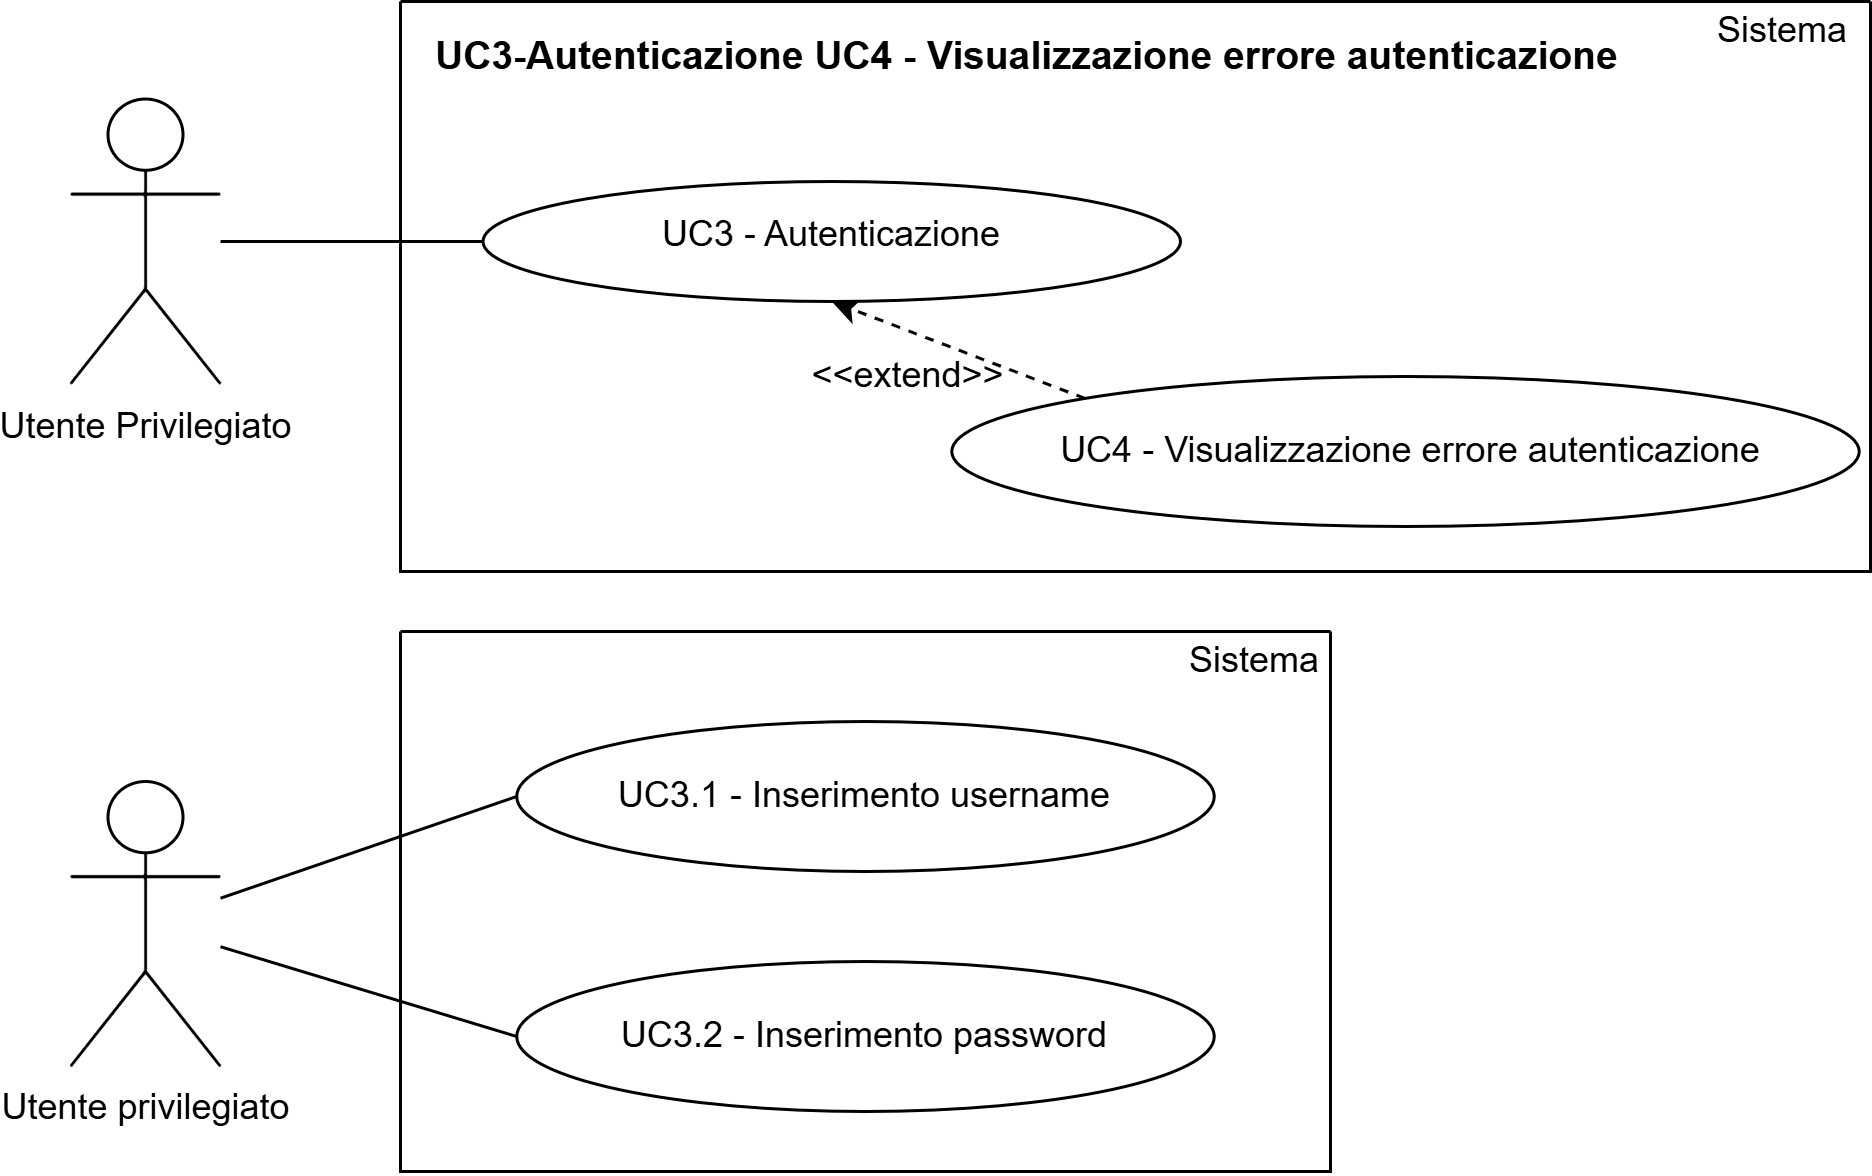
\includegraphics[width=0.5\linewidth]{UC3-UC4image.png}
    \caption{UC3 - Autenticazione | UC4 - Visualizzazione errore autenticazione}
    \label{fig:UC3 e UC4}
\end{figure}
%%%%%%%%%%%%%%%%%%%%%%%%%%%%%%%%%%%%%%%%%%%%%%%%%%%%%%%%%%%%%%%%%%%%%%%%%%%
\subsubsection{\textbf{UC3.1 - Inserimento username}}
\begin{itemize}
     \item \textbf{Attore Principale:} Utente Privilegiato.
     \item \textbf{Precondizioni:} 
            \begin{itemize}
                \item L'utente privilegiato sta eseguendo l'autenticazione (UC3).
            \end{itemize}
     \item \textbf{Postcondizioni:} Il nome utente è stato inserito nel campo dati preposto.
     \item \textbf{Scenario Principale:}
        \begin{enumerate}
            \item L'utente privilegiato inserisce il suo username nell'apposito campo dati.
        \end{enumerate}
     \item \textbf{User story associata:} Come utente privilegiato voglio poter inserire lo username al fine di eseguire l'accesso.
\end{itemize}
%%%%%%%%%%%%%%%%%%%%%%%%%%%%%%%%%%%%%%%%%%%%%%%%%%%%%%%%%%%%%%%%%%%%%%%%%%%
\subsubsection{\textbf{UC3.2 - Inserimento password}}
\begin{itemize}
     \item \textbf{Attore Principale:} Utente Privilegiato.
     \item \textbf{Precondizioni:} 
        \begin{itemize}
            \item L'utente privilegiato sta eseguendo l'autenticazione (UC3).
        \end{itemize}
     \item \textbf{Postcondizioni:} La password è stata inserita nel campo dati preposto.
     \item \textbf{Scenario Principale:}
        \begin{enumerate}
            \item L'utente privilegiato inserisce la sua password nell'apposito campo dati.
        \end{enumerate}
     \item \textbf{User story associata:} Come utente privilegiato voglio poter inserire la password al fine di eseguire l'accesso.
\end{itemize}
%%%%%%%%%%%%%%%%%%%%%%%%%%%%%%%%%%%%%%%%%%%%%%%%%%%%%%%%%%%%%%%%%%%%%%%%%%%
\subsubsection{\textbf{UC4 - Visualizzazione errore autenticazione}}
\begin{itemize}
    \item \textbf{Attore Principale:} Utente privilegiato.
    \item \textbf{Precondizioni:}
        \begin{itemize}
            \item Il sistema è operativo e accessibile.
            \item L'utente privilegiato ha inserito una combinazione non valida di username e password.
            \item L'autenticazione (UC3) è fallita.
        \end{itemize}
    \item \textbf{Postcondizioni:}
        \begin{itemize}
            \item L’utente privilegiato visualizza un messaggio di errore.
            \item L’utente privilegiato può correggere le credenziali e provare ad effettuare nuovamente l'autenticazione.
        \end{itemize}
    \item \textbf{Scenario Principale:}
        \begin{enumerate}
            \item L'utente privilegiato inserisce le credenziali e effettua l'accesso.
            \item Il sistema verifica la credenziali inserite e se una delle due o entrambe non sono valide fa visualizzare un messaggio di errore.
        \end{enumerate}
    \item \textbf{User story associata:} Come utente privilegiato, voglio poter visualizzare un messaggio di errore nel caso avessi inserito le credenziali errate.
\end{itemize}
%%%%%%%%%%%%%%%%%%%%%%%%%%%%%%%%%%%%%%%%%%%%%%%%%%%%%%%%%%%%%%%%%%%%%%%%%%%
\subsubsection{\textbf{UC1 - Visualizzazione dashboard}}
\begin{itemize}
    \item \textbf{Attore Principale:} Utente privilegiato.
    \item \textbf{Precondizioni:} Il sistema è operativo e accessibile.
    \item \textbf{Postcondizioni:} L'utente privilegiato è in grado di visualizzare una mappa geografica, con i sensori GPS aggiornati in tempo reale (marker), i vari punti di interesse e le pubblicità offerte agli utenti.
    \item \textbf{Scenario Principale:}
        \begin{enumerate}
            \item L'utente privilegiato accede alla piattaforma di visualizzazione della dashboard.
            \item Il sistema mette a disposizioni tutte le informazioni storicizzate e ricevute dai sensori, distribuiti su una mappa tramite marker.
        \end{enumerate}
    \item \textbf{User story associata:} Come utente privilegiato, voglio accedere alla dashboard per visualizzare in tempo reale i mezzi che ho messo a noleggio (sensori GPS), i punti di interesse che usufruiscono di questo servizio e le inserzioni che vengono generate per gli utenti che hanno effettuato il noleggio.
\end{itemize}
\begin{figure}[ht]
    \centering
    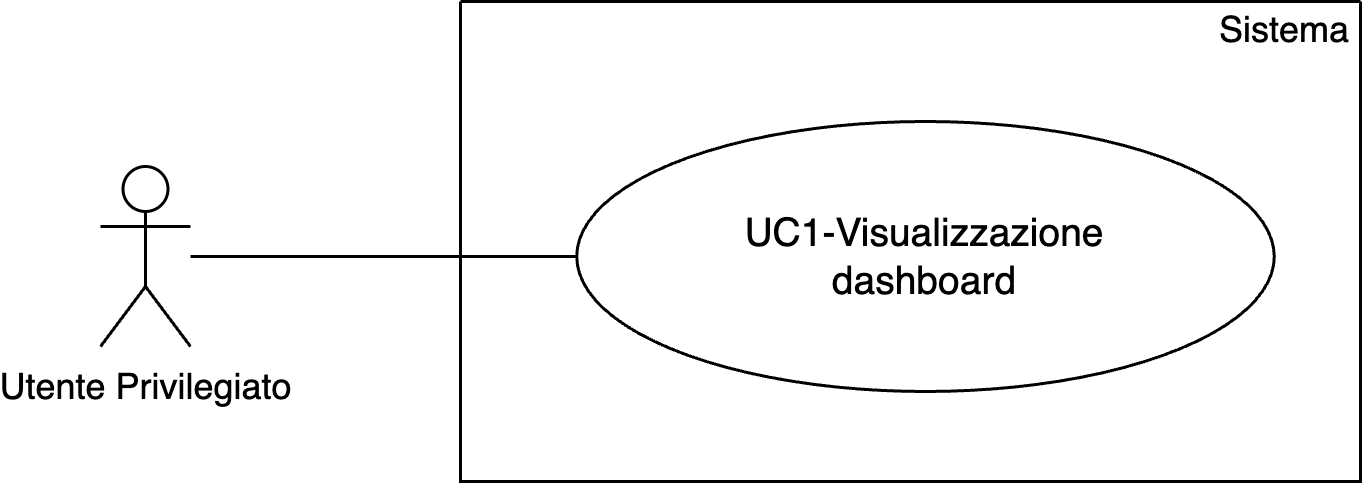
\includegraphics[width=0.5\linewidth]{UC1image.png}
    \caption{UC1 - Visualizzazione Dashboard}
    \label{fig:UC1}
\end{figure}
%%%%%%%%%%%%%%%%%%%%%%%%%%%%%%%%%%%%%%%%%%%%%%%%%%%%%%%%%%%%%%%%%%%%%%%%%%%
\subsubsection{\textbf{UC1.1 - Visualizzazione dettagli dei marker sulla mappa}}
\begin{itemize}
     \item \textbf{Attore Principale:} Utente Privilegiato.
     \item \textbf{Precondizioni:}
        \begin{itemize}
    		\item L'utente privilegiato ha effettuato l'accesso e sta      visualizzando la dashboard (UC3 e UC1).
        \end{itemize}
     \item \textbf{Postcondizioni:} L'utente privilegiato è in grado di ottenere informazioni più dettagliate dell'utente selezionando il marker visibile sulla mappa.
     \item \textbf{Scenario Principale:}
        \begin{itemize}
            \item L'utente privilegiato ha accesso alla dashboard con la mappa interattiva (UC3 e UC1).
            \item L'utente privilegiato seleziona un marker per vederne le informazioni più dettagliate.
            \item Il sistema mette a disposizione il dato più recententemente archiviato per quel marker.
        \end{itemize}
     \item \textbf{User story associata:}
     Come utente privilegiato voglio selezionare i vari marker, che indicano i mezzi di trasporto, presenti sulla mappa, in modo da vedere i dettagli sulla posizione e sull'utente che sta utilizzando il mezzo.
\end{itemize}
\begin{figure}[ht]
    \centering
    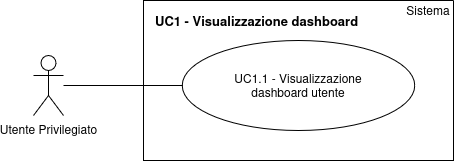
\includegraphics[width=0.5\linewidth]{UC1.1image.png}
    \caption{UC1.1 - Visualizzazione dettagli dei marker sulla mappa}
    \label{fig:UC1.1}
\end{figure}
%%%%%%%%%%%%%%%%%%%%%%%%%%%%%%%%%%%%%%%%%%%%%%%%%%%%%%%%%%%%%%%%%%%%%%%%%%%
\subsubsection{\textbf{UC1.2 - Visualizzazione annunci sulla mappa}}
\begin{itemize}
    \item \textbf{Attore Principale:} Utente privilegiato.
    \item \textbf{Precondizioni:} 
        \begin{itemize}
    	\item L'utente privilegiato ha effettuato l'accesso e sta          visualizzando la dashboard (UC3 e UC1).
        \end{itemize}
    \item \textbf{Postcondizioni:} L'Utente privilegiato visualizzerà un annuncio personalizzato del punto di interesse in base ai dati dell'utente che passa vicino a quel punto.
    \item \textbf{Scenario Principale:} 
        \begin{itemize}
    	\item Un utente, mentre si muove sulla mappa, passa nell'area      di un punto di interesse.
    	\item Il sistema elabora le informazioni dell'utente e del         punto di interesse per generare il testo dell'eventuale            annuncio.
	\end{itemize}
    \item \textbf{User story associata:} Come utente privilegiato voglio visualizzare gli annunci pubblicitari che arrivano ai vari utenti.
\end{itemize}
\begin{figure}[ht]
    \centering
    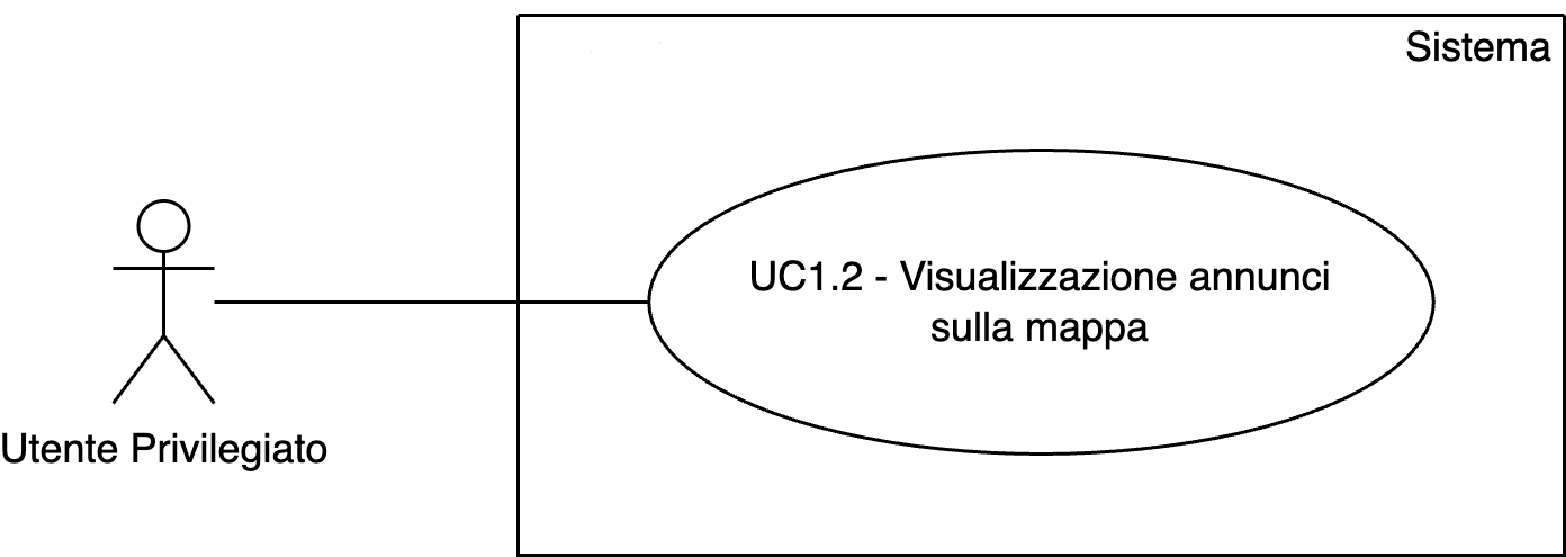
\includegraphics[width=0.5\linewidth]{UC1.2image.png}
    \caption{UC1.2 - Visualizzazione annunci sulla mappa}
    \label{fig:UC1.2}
\end{figure}
%%%%%%%%%%%%%%%%%%%%%%%%%%%%%%%%%%%%%%%%%%%%%%%%%%%%%%%%%%%%%%%%%%%%%%%%%%%
\subsubsection{\textbf{UC1.3 - Visualizzazione dettagli dei punti di interesse sulla mappa}}
\begin{itemize}
     \item \textbf{Attore Principale:} Utente Privilegiato.
     \item \textbf{Precondizioni:}
        \begin{itemize}
    		\item L'utente privilegiato ha effettuato l'accesso e sta visualizzando la dashboard (UC3 e UC1).
        \end{itemize}
     \item \textbf{Postcondizioni:} L'utente privilegiato è in grado di ottenere informazioni più dettagliate selezionando il punto di interesse visibile sulla mappa.
     \item \textbf{Scenario Principale:}
        \begin{itemize}
            \item L'utente privilegiato seleziona un punto di interesse per vederne le informazioni più dettagliate.
            \item Il sistema mette a disposizione il dato più recententemente archiviato per quel punto di interesse.
        \end{itemize}
     \item \textbf{User story associata:}
     Come utente privilegiato voglio selezionare i vari punti di interesse presenti sulla mappa, in modo da vederne i dettagli.
\end{itemize}
\begin{figure}[ht]
    \centering
    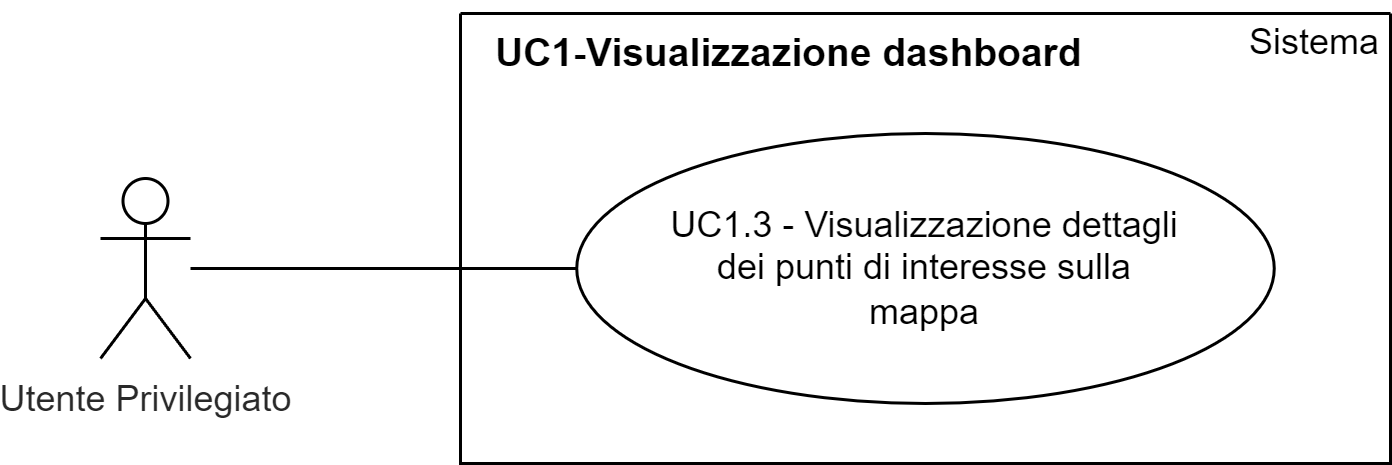
\includegraphics[width=0.5\linewidth]{UC1.3image.png}
    \caption{UC1.3 - Visualizzazione dettagli punti di interesse sulla mappa}
    \label{fig:UC1.3}
\end{figure}
%%%%%%%%%%%%%%%%%%%%%%%%%%%%%%%%%%%%%%%%%%%%%%%%%%%%%%%%%%%%%%%%%%%%%%%%%%%
\subsubsection{\textbf{UC1.3.1 - Visualizzazione area del punto di interesse}}
\begin{itemize}
     \item \textbf{Attore Principale:} Utente Privilegiato.
     \item \textbf{Precondizioni:}
        \begin{itemize}
            \item L'utente privilegiato ha effettuato l'accesso e sta visualizzando la dashboard (UC3 e UC1).
            \item L'utente privilegiato ha selezionato un punto di interesse (UC1.3).
        \end{itemize}
     \item \textbf{Postcondizioni:} L'utente privilegiato è in grado di visualizzare l'area di influenza di un punto di interesse visibile sulla mappa.
     \item \textbf{Scenario Principale:}
        \begin{enumerate}
            \item Il sistema genera l'area di influenza del punto di interesse selezionato e la mostra sulla mappa.
        \end{enumerate}
     \item \textbf{User story associata:}
     Come utente privilegiato voglio vedere l'area di influenza di ogni punto di interesse presente sulla mappa.
\end{itemize}
%\begin{figure}[ht]
%    \centering
%    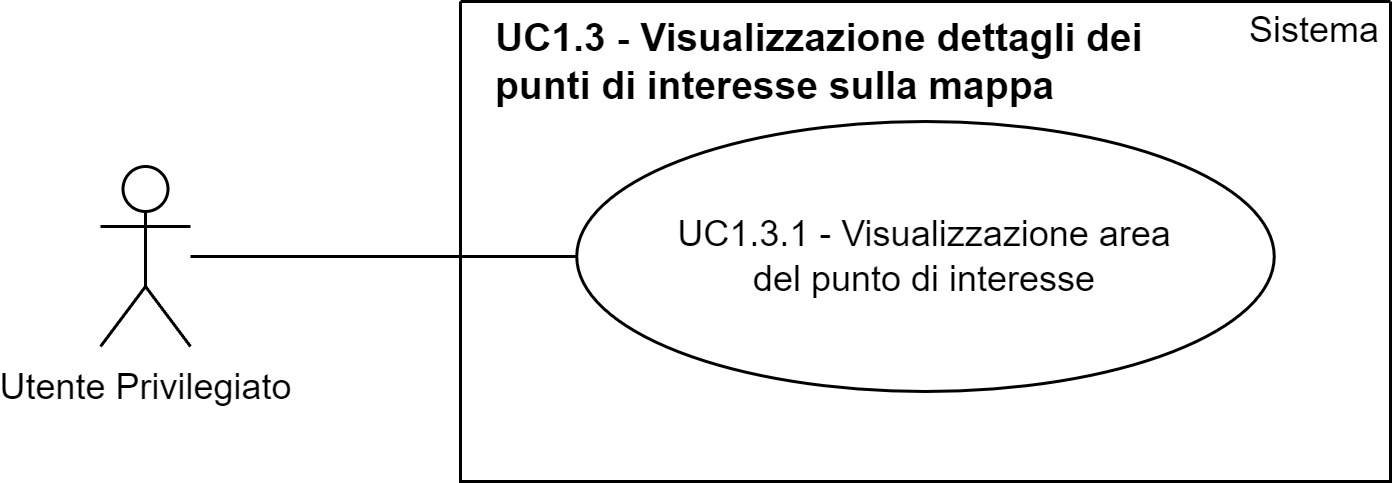
\includegraphics[width=0.5\linewidth]{UC1.3.1image.png}
%    \caption{UC1.3.1 - Visualizzazione area del punto di interesse}
%    \label{fig:UC1.3.1}
%\end{figure}
%%%%%%%%%%%%%%%%%%%%%%%%%%%%%%%%%%%%%%%%%%%%%%%%%%%%%%%%%%%%%%%%%%%%%%%%%%%
 \subsubsection{\textbf{UC1.3.2 - Visualizzazione informazioni del punto di interesse}}
 \begin{itemize}
     \item \textbf{Attore Principale:} Utente Privilegiato
     \item \textbf{Precondizioni:}
       \begin{itemize}
            \item L'utente privilegiato ha effettuato l'accesso e sta visualizzando la dashboard (UC3 e UC1).
            \item L'utente privilegiato ha selezionato un punto di interesse (UC1.3).
       \end{itemize}
     \item \textbf{Postcondizioni:} L'utente privilegiato è in grado di visualizzare le informazioni specifiche del punto di interesse selezionato.
     \item \textbf{Scenario Principale:}
        \begin{enumerate}
            \item Il sistema riporta le informazioni del punto di interesse selezionato e li mostra nella dashboard.
        \end{enumerate}
     \item \textbf{User story associata:} Come utente privilegiato voglio visualizzare le informazioni di un punto di interesse presente sulla mappa. 
 \end{itemize}
\begin{figure}[ht]
    \centering
    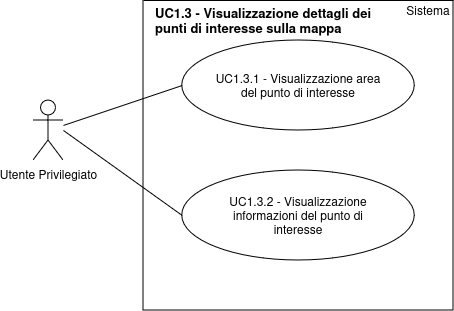
\includegraphics[width=0.5\linewidth]{UC1.3.1-UC1.3.2image.png}
    \caption{UC1.3.1 - Visualizzazione area del punto di interesse -- UC1.3.2 - Visualizzazione informazioni del punto di interesse}
    \label{fig:UC1.3.1-UC1.3.2}
\end{figure}
%%%%%%%%%%%%%%%%%%%%%%%%%%%%%%%%%%%%%%%%%%%%%%%%%%%%%%%%%%%%%%%%%%%%%%%%%%%
\subsubsection{\textbf{UC2 - Visualizzazione annuncio}}
\begin{itemize}
    \item \textbf{Attore Principale:} Utente
    \item \textbf{Precondizioni:} 
        \begin{itemize}
    	\item Il sistema è operativo e accessibile.
    	\item Un utente entra nell'area di un punto di interesse.
        \end{itemize}
    \item \textbf{Postcondizioni:} L'Utente visualizzerà un eventuale messaggio contenente un annuncio personalizzato in base ai suoi dati personali e al punto di interesse.
    \item \textbf{Scenario Principale:} 
        \begin{enumerate}
            \item Un utente, mentre si muove sulla mappa, passa    nell'area di un punto di interesse.
            \item Il sistema elabora le informazioni dell'utente e del punto di interesse per generare il testo dell'eventuale annuncio.
            \item Il sistema invia all'utente il messaggio contenente l'annuncio se questo è stato generato.
        \end{enumerate}
    \item \textbf{User story associata:} Come utente voglio visualizzare gli annunci pubblicitari personalizzati che mi arrivano.
\end{itemize}
\begin{figure}[ht]
    \centering
    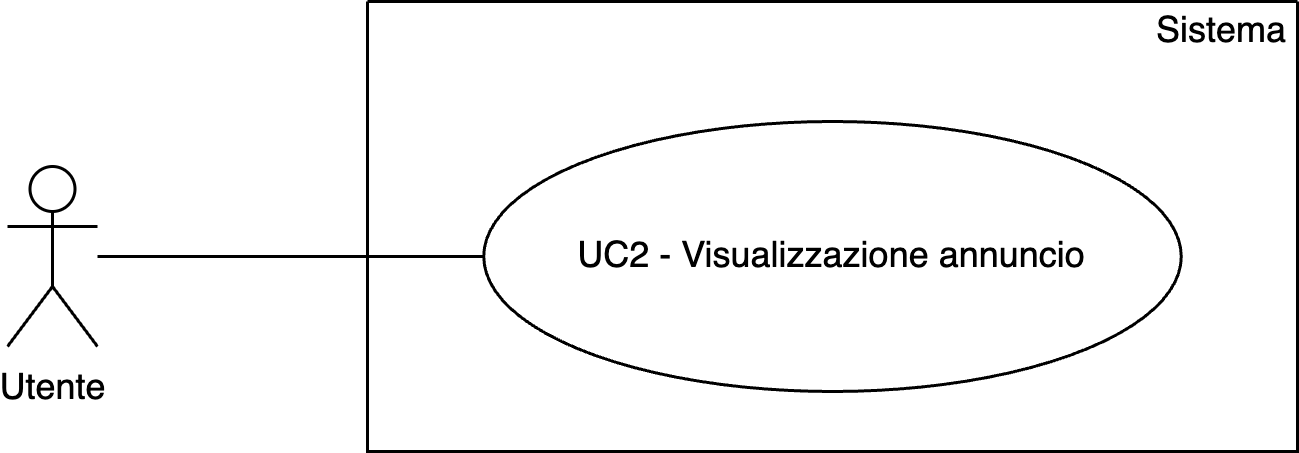
\includegraphics[width=0.5\linewidth]{UC2image.png}
    \caption{UC2 - Visualizzazione annuncio}
    \label{fig:UC2}
\end{figure}
%%%%%%%%%%%%%%%%%%%%%%%%%%%%%%%%%%%%%%%%%%%%%%%%%%%%%%%%%%%%%%%%%%%%%%%%%%%
\subsubsection{\textbf{UC5 - Trasmissione dati geoposizionali}}
\begin{itemize}
    \item \textbf{Attore Principale:} Sensore
    \item \textbf{Precondizioni:} 
        \begin{itemize}
    	\item Il sensore è attivo e connesso al sistema.
        \end{itemize}
    \item \textbf{Postcondizioni:} Il sistema memorizza ed elabora i dati ricevuti dal sensore.
    \item \textbf{Scenario Principale:} 
        \begin{enumerate}
            \item Il sensore di tipo GPS effettua un rilevamento della posizione geografica dell'utente(latitudine e longitudine).
            \item Il sensore GPS formatta il messaggio da trasmettere al sistema contenente l’identificativo dell'utente e le coordinate geografiche individuate.
            \item Il sensore GPS emette il messaggio al sistema.
        \end{enumerate}
    \item \textbf{User story associata:} Come Sensore GPS, desidero trasmettere i rilevamenti di posizione al sistema.

\end{itemize}
\begin{figure}[ht]
    \centering
    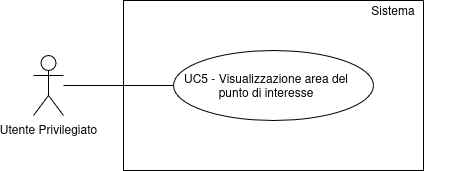
\includegraphics[width=0.5\linewidth]{UC5image.png}
    \caption{UC5 - Trasmissione dati geoposizionali}
    \label{fig:UC5}
\end{figure}
%%%%%%%%%%%%%%%%%%%%%%%%%%%%%%%%%%%%%%%%%%%%%%%%%%%%%%%%%%%%%%%%%%%%%%%%%%%

%%%%%%%%%%%%%%%%%%%%%%%%%%%%%%%%%%%%%%%%%%%%%%%%%%%%%%%%%%%%%%%%%%%%%%%%%%%

\newpage
\section{Requisiti}
%sicuramente da suddividere intenamente tra obbligatori, desiderabilli e opzionali

\subsection{Requisiti funzionali}

% Definisci una nuova colonna centrata con larghezza fissa
\newcolumntype{C}[1]{>{\centering\arraybackslash}m{#1}}

\begin{table}[H]
\centering
\renewcommand{\arraystretch}{1.5}
\begin{tabular}{|>{\centering\arraybackslash}m{2.7cm}|>{\centering\arraybackslash}m{2.7cm}|>{\centering\arraybackslash}m{6cm}|>{\centering\arraybackslash}m{2.1cm}|}
%\begin{tabular}{|>{\vspace{5pt}}C{2.7cm}<{\vspace{5pt}}|>{\vspace{5pt}}C{2.7cm}<{\vspace{5pt}}|>{\vspace{5pt}}m{6cm}<{\vspace{5pt}}|>{\vspace{5pt}}C{2.1cm}<{\vspace{5pt}}|}
\hline
\textbf{Id. Requisito} & \textbf{Importanza} & \textbf{Descrizione} & \textbf{Fonti}\\
\hline
 RF01 &  Obbligatorio &  L'utente privilegiato deve poter visualizzare la dashboard composta da una mappa interattiva con i vari marker e punti di interesse su di essa. &  Capitolato, UC1\\
\hline
RF02 & Obbligatorio & L'utente privilegiato deve poter visualizzare i dettagli provenienti da un determinato marker. & Interna, UC1.1\\
\hline
RF03 & Obbligatorio & L'utente privilegiato deve poter visualizzare gli annunci pubblicitari provenienti da un determinato punto di interesse. & Capitolato, UC1.2\\
\hline
RF04 & Obbligatorio & L'utente privilegiato deve poter visualizzare i dettagli provenienti da un determinato punto di interesse. & Interna, UC1.3\\
\hline
RF05 & Opzionale & L'utente privilegiato deve poter visualizzare l'area di influenza di un punto di interesse selezionato. & Interna, UC1.3.1\\
\hline
RF06 & Opzionale & L'utente deve poter visualizzare l'annuncio pubblicitario proveniente dal punto di interesse situato nell'area che sta attraversando. & Capitolato, UC2\\
\hline
RF07 & Obbligatorio & L'utente privilegiato deve poter effetturare l'accesso per visualizzare la dashboard. & Capitolato, UC3, UC3.1, UC3.2\\
\hline
RF08 & Obbligatorio & L'utente privilegiato deve poter visualizzare un messaggio di errore nel caso le credenziali inserite durante l'accesso non siano riconosciute. & Capitolato, UC4\\
\hline
RF09 & Obbligatorio & Il sensore deve essere in grado di trasmettere i dati in tempo reale al sistema. & Capitolato, UC5\\
\hline
RF10 & Obbligatorio & L'utente privilegiato deve poter visualizzare le informazioni del singolo punto di interesse & Capitolato, UC1.3.2\\
\hline
\end{tabular}
\caption{Requisiti funzionali}
\end{table}

%---------------------------------------------------------------------------------------------------------------------------------------------
\newpage
\subsection{Requisiti di qualità}

\begin{table}[H]
\centering
\renewcommand{\arraystretch}{1.5}
\begin{tabular}{|>{\centering\arraybackslash}m{2.7cm}|>{\centering\arraybackslash}m{2.7cm}|>{\centering\arraybackslash}m{6cm}|>{\centering\arraybackslash}m{2.1cm}|}
%\begin{tabular}{|>{\vspace{5pt}}C{2.7cm}<{\vspace{5pt}}|>{\vspace{5pt}}C{2.7cm}<{\vspace{5pt}}|>{\vspace{5pt}}m{6cm}<{\vspace{5pt}}|>{\vspace{5pt}}C{2.1cm}<{\vspace{5pt}}|}
\hline
\textbf{Id. Requisito} & \textbf{Importanza} & \textbf{Descrizione} & \textbf{Fonti}\\
\hline
RQ01 & Obbligatorio & Presentare documento di analisi dei requisiti d'analisi contenente i diagrami UML relativi ai casi d'uso. & Capitolato\\
\hline
RQ02 & Obbligatorio & Devono essere rispettate tutte le norme definite nel documento \textit{Norme\_di\_Progetto.pdf}, nell'apposita sezione Analisi dei Requisiti. & Interna\\
\hline
RQ03 & Obbligatorio & Deve essere fornita documentazione riguardante le scelte di design del prodotto, con la motivazione delle scelte implementative e tecnologiche. & Capitolato, Verbale Esterno 2024-11-25\\
\hline
RQ04 & Obbligatorio & È necessaria la realizzazione di test che dimostrino il corretto funzionamento dei servizi e delle funzionalità previste, con una copertura minima dell'80\% e documentata tramite un report.  & Capitolato\\
\hline
RQ05 & Obbligatorio & È richiesto che il sistema venga testato nella sua interezza tramite test end-to-end, anche non automatizzati.  & Capitolato\\
\hline
RQ06 & Obbligatorio & La documentazione dovrà riguardare anche problemi aperti ed eventuali possibili soluzioni da approfondire in futuro.  & Capitolato\\
\hline
\end{tabular}
\caption{Requisiti di qualità}
\end{table}

%---------------------------------------------------------------------------------------------------------------------------------------------
\newpage
\subsection{Requisiti di vincolo}

\begin{table}[H]
\centering
\renewcommand{\arraystretch}{1.5}
\begin{tabular}{|>{\centering\arraybackslash}m{2.7cm}|>{\centering\arraybackslash}m{2.7cm}|>{\centering\arraybackslash}m{6cm}|>{\centering\arraybackslash}m{2.1cm}|}
%\begin{tabular}{|>{\vspace{5pt}}C{2.7cm}<{\vspace{5pt}}|>{\vspace{5pt}}C{2.7cm}<{\vspace{5pt}}|>{\vspace{5pt}}m{6cm}<{\vspace{5pt}}|>{\vspace{5pt}}C{2.1cm}<{\vspace{5pt}}|}
\hline
\textbf{Id. Requisito} & \textbf{Importanza} & \textbf{Descrizione} & \textbf{Fonti}\\
\hline
RV01 & Obbligatorio &  Per sviluppare il prodotto occorrerà utilizzare il linguaggio Python. & Interna\\
\hline 
RV02 & Obbligatorio & L'ambiente di sviluppo e di deployment deve utilizzare la tecnologia multi-container, in particolare Docker Compose. & Capitolato, Interna\\
\hline
RV03 & Obbligatorio & I rilevamenti dei sensori geoposizionali
devono essere memorizzati nel corretto formato in un time series database, nel nostro sistema sarà Clickhouse. & Capitolato, Interna \\
\hline
RV04 & Obbligatorio & I dati raccolti e processati devono essere visualizzabili su una piattaforma di dashboard interattiva, come Grafana. & Capitolato, Interna\\
\hline
RV05 & Obbligatorio & Le coordinate generate per la simulazione di un utente che segue un percorso devono essere realistiche. & Capitolato\\
\hline
\end{tabular}

\caption{Requisiti di vincolo}
\end{table}


%---------------------------------------------------------------------------------------------------------------------------------------------
\newpage
\subsection{Requisiti prestazionali}

\begin{table}[H]
\centering
\renewcommand{\arraystretch}{1.5}
\begin{tabular}{|>{\centering\arraybackslash}m{2.7cm}|>{\centering\arraybackslash}m{2.7cm}|>{\centering\arraybackslash}m{6cm}|>{\centering\arraybackslash}m{2.1cm}|}
%\begin{tabular}{|>{\vspace{5pt}}C{2.7cm}<{\vspace{5pt}}|>{\vspace{5pt}}C{2.7cm}<{\vspace{5pt}}|>{\vspace{5pt}}m{6cm}<{\vspace{5pt}}|>{\vspace{5pt}}C{2.1cm}<{\vspace{5pt}}|}
\hline
\textbf{Id. Requisito} & \textbf{Importanza} & \textbf{Descrizione} & \textbf{Fonti}\\
\hline
RP01 & Obbligatorio &  Il sistema deve gestire inizialmente la generazione di un dato geoposizionale ogni 5 secondi e un utente noleggiatore del mezzo & Capitolato\\
\hline
RP02 & Obbligatorio &  Il sistema deve sopportare ingenti quantità do dato in INSERT & Capitolato\\
\hline
\end{tabular}
\caption{Requisiti prestazionali}
\end{table}

%---------------------------------------------------------------------------------------------------------------------------------------------


\newpage
\section{Tracciamento Requisiti}

\begin{table}[H]
\centering
\begin{tabular}{|>{\vspace{5pt}}C{2.7cm}<{\vspace{5pt}}|>{\vspace{5pt}}C{2.7cm}<{\vspace{5pt}}|}
\hline
\textbf{Fonte} & \textbf{Id. Requisiti}\\
\hline
Capitolato & RF01 \linebreak RF03 \linebreak RF06 \linebreak RF07 \linebreak RF08 \linebreak RF09 \linebreak RF10 \linebreak RQ01  \linebreak RQ03 \linebreak RV02 \linebreak RV03 \linebreak RV04 \linebreak RP01 \linebreak RQ04 \\
\hline
Interna & RF02 \linebreak RF04 \linebreak RF05 \linebreak RV01 \linebreak RV02 \linebreak RV03 \linebreak RV04 \linebreak RQ02 \\
\hline
\end{tabular}
\caption{Tracciamento Fonte-Requisiti}
\end{table}

%---------------------------------------------------------------------------------------------------------------------------------------------

\subsection{Riepilogo}
\begin{table}[H]
\centering
\begin{tabular}{|>{\vspace{4pt}}C{2.4cm}<{\vspace{4pt}}|>{\vspace{4pt}}C{2.3cm}<{\vspace{4pt}}|>{\vspace{4pt}}C{2.3cm}<{\vspace{4pt}}|>{\vspace{4pt}}C{2.3cm}<{\vspace{4pt}}|>{\vspace{4pt}}C{1.4cm}<{\vspace{4pt}}|}
\hline
\textbf{Tipologia} & \textbf{Obbligatori} & \textbf{Desiderabili} & \textbf{Opzionali} & \textbf{Totale}\\
\hline
Funzionali & 7 & - & 2 & 9\\
\hline
Di qualità & 6 & - & - & 6 \\
\hline
Di vincolo & 5 & - & - & 5 \\
\hline
Prestazionali & 2 & - & - & 2 \\
\hline
Totale & 20 & - & 2 & 22 \\
\hline
\end{tabular}
\caption{Riepilogo}
\end{table}

\end{justify}
\end{document}
